\input ../SlidePreamble
\input ../preamble


\begin{document}

{\Huge

  \centerline{\bf TTIC 31230, Fundamentals of Deep Learning}
  \bigskip
  \centerline{David McAllester, Autumn 2022}
  \vfill
  \vfil
  \centerline{DALL$\cdot$E-2}
  \vfill
  \vfill

\slide{DALL$\cdot$E-2}

\centerline{\hfill \includegraphics[width = 4.5in]{\images/DALLEpanda} \hfill 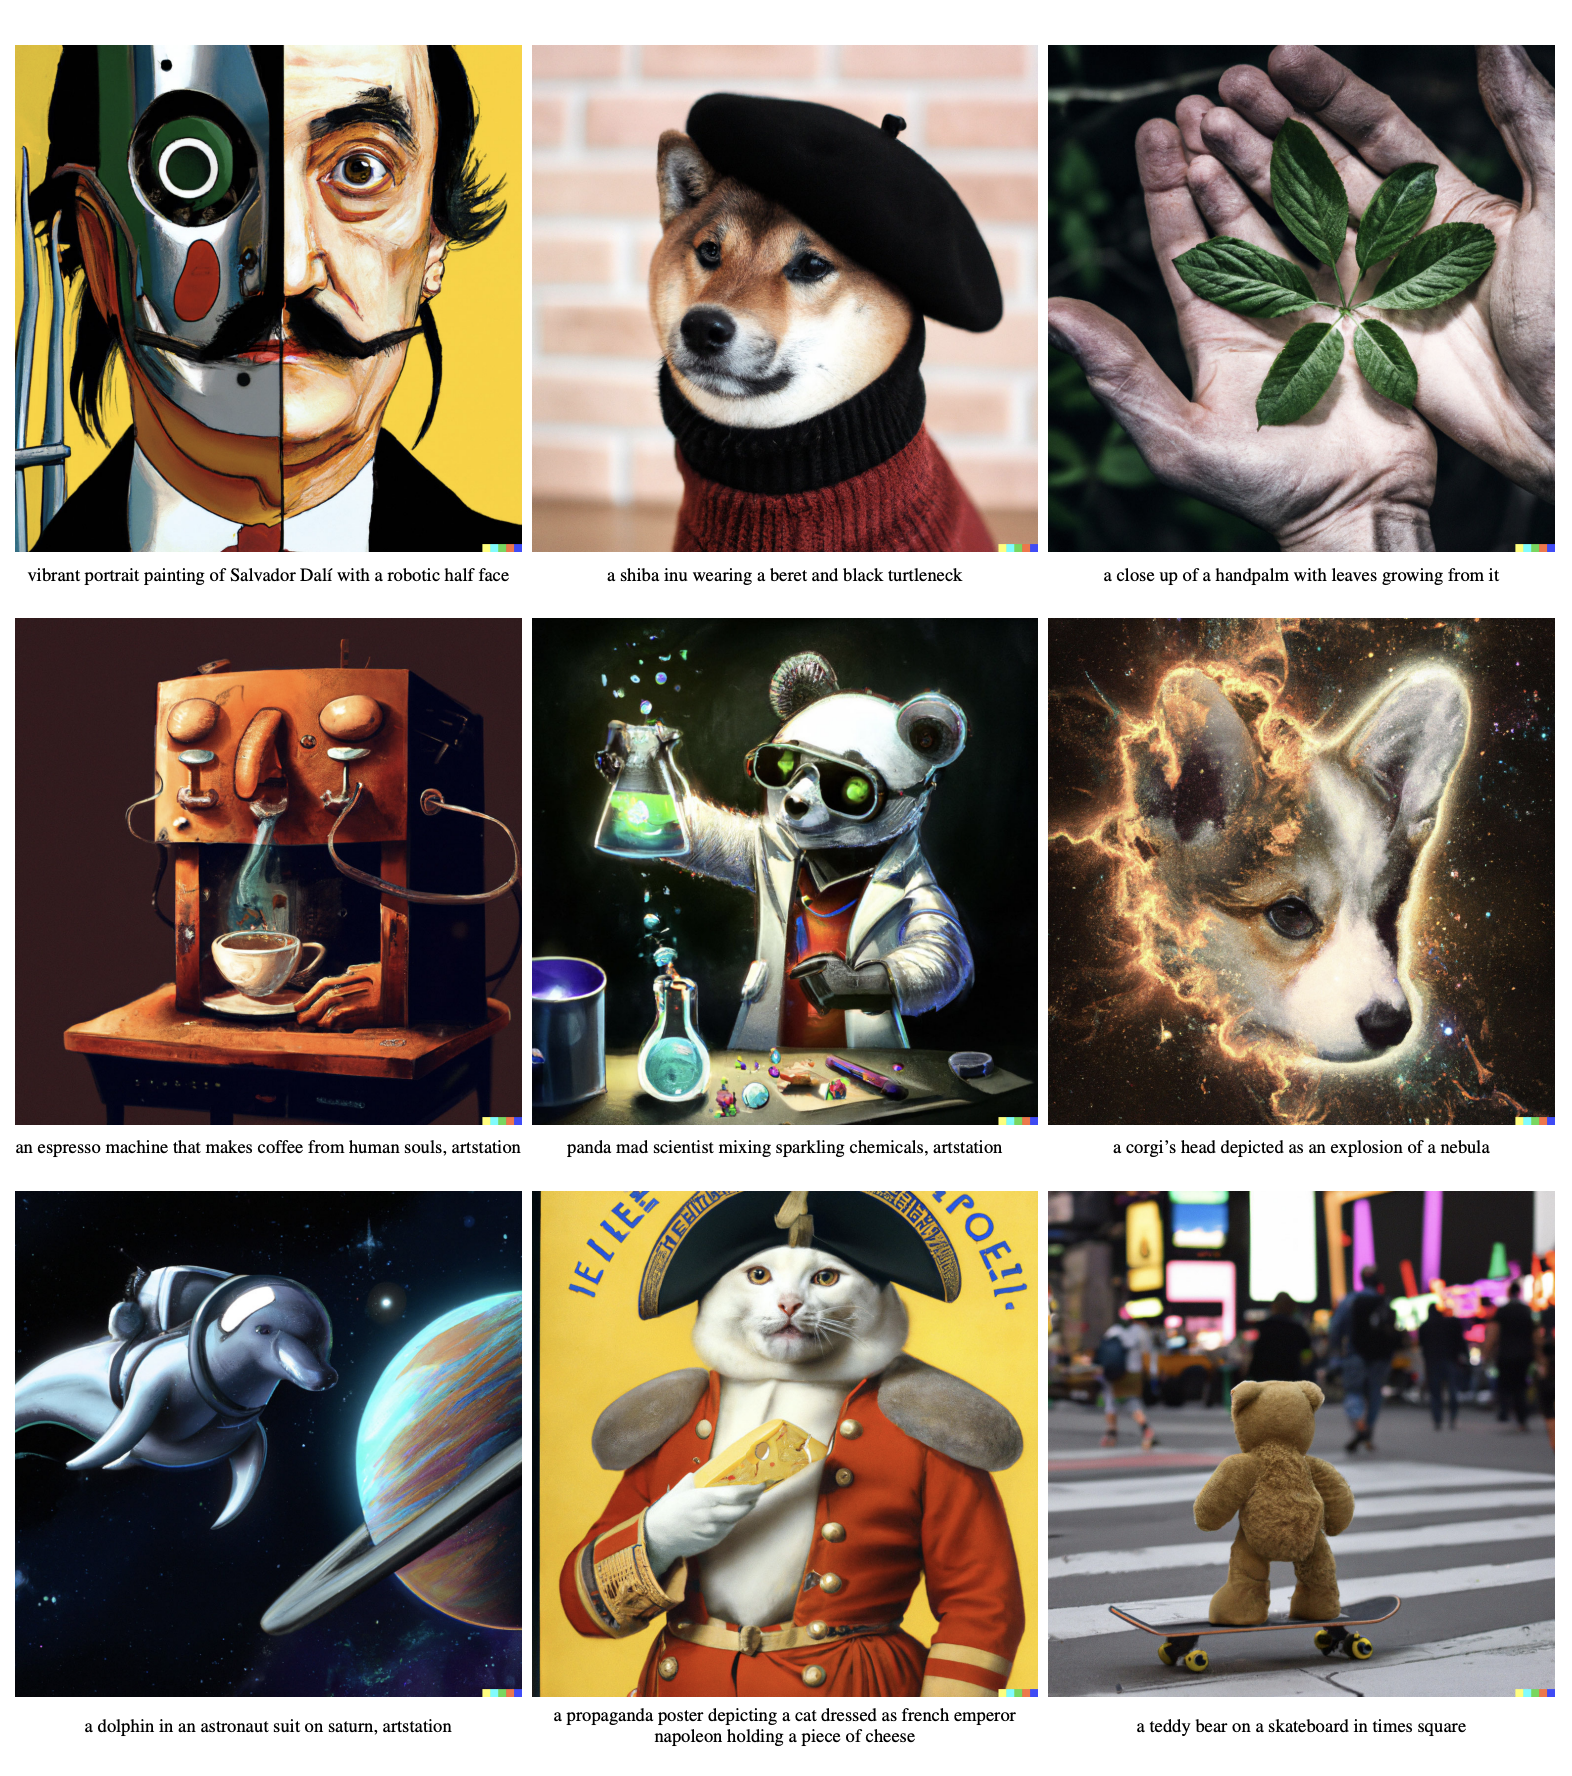
\includegraphics[width = 3in]{\images/DALLE2}}

\slide{Conditional Cross Entropy Loss}

$$\Phi^* = \argmin_\Phi\;E_{(x,y) \sim \pop} \;-\ln P_\Phi(y|x)$$

\vfill
In DALLE we have that $x$ is text and $y$ is an image.

\vfill
We need to formulate {\bf conditional diffusion models} in a way that supports conditioning images on text.

\vfill
We would like to both be able to compute (or upper bound bound) $P_\Phi(y|x)$ and also to generate $y$ from $P_\Phi(y|x)$.

\slide{DALL$\cdot$E-2}

DALLE combines diffusion models with CLIP.

\vfill

\centerline{\includegraphics[width = 8in]{\images/DALLE2a}}

\slide{CLIP Does Contrastive Coding}

\centerline{\includegraphics[height= 4in]{\images/CLIPTraining}}


\slidetwo{GLIDE: Towards Photorealistic Image Generation ...}
         {Nichol, Dhariwal, Ramesh, et al., March 2022}

For text $x$ let $C_T(x) \in R^I$ be the CLIP embedding of $x$.

\vfill
For a (possibly noised) image $z$ let $C_I(z)$ be a CLIP embedding of $z$.

\vfill
Here CLIP is re-trained to handle noised images.

A first approach to is to define the update direction by

$\epsilon(z_\ell,

\slide{END}
}
\end{document}
